\ExerciseGroupsStart
\ExerciseSection

\begin{enumerate}
\def\labelenumi{\arabic{enumi})}
\tightlist
\item
  * a) Let \(f\) be a homomorphism of the additive group \(\mathbf{R}\) into itself. Show that, if the graph of \(f\) is not dense in \(\mathbf{R}^2\) , \(f\) is of the form \(x \to ax\) {[}consider the closure in \(\mathbf{R}^2\) of the graph of \(f\) , and use the structure theorem for closed subgroups of \(\mathbf{R}^2\) (Chapter VII, § 1, no. 2, Theorem 2){]}. * {[}Compare with Chapter VI, § 1, Exercise 12 b) and Chapter IV, § 6, Exercise 2.{]}
\end{enumerate}

\begin{enumerate}
\def\labelenumi{\alph{enumi})}
\setcounter{enumi}{1}
\tightlist
\item
  If the graph of f is dense in \(R^{2}\) , the inverse image of the topology of \(R^{2}\) under the mapping \(x \to (x, f(x))\) is compatible with the group structure of R and is strictly finer than the usual topology of R. If moreover f is injective, the inverse image under f of the usual topology of R is compatible with the group structure of R and is not comparable with the usual topology of R.
\end{enumerate}

\begin{enumerate}
\def\labelenumi{\arabic{enumi})}
\setcounter{enumi}{1}
\tightlist
\item
  Let \(\mathfrak{C}\) be a Hausdorff topology on \(\mathbf{R}\) , compatible with the group structure of \(\mathbf{R}\) and strictly coarser than the usual topology \(\mathfrak{C}_0\) .
\end{enumerate}

\begin{enumerate}
\def\labelenumi{\alph{enumi})}
\item
  Show that every open neighbourhood of o with respect to \(\mathfrak{C}\) is unbounded in \(\mathbf{R}\) (note that a Hausdorff topology which is coarser than the topology of a compact space must coincide with the latter).
\item
  Let \(V \neq R\) be a symmetric open neighbourhood of o with respect to \(\mathfrak{C}\), and let W be a symmetric open neighbourhood of o with respect to \(\mathfrak{C}\) such that \(W + W \subset V\) . Show that if a is the length of the component of V (with respect to \(\mathfrak{C}_{0}\) ) which contains o, then every component (with respect to \(\mathfrak{C}_{0}\) ) of W has length \(\leqslant a\) . Moreover, the set of lengths of components of the interior of R - W (with respect to \(\mathfrak{C}_{0}\) ) is bounded {[}use a) and the fact that there exists a symmetric open neighbourhood \(W_{1}\) of o with respect to \(\mathfrak{C}\) such that \(W_{1} + W_{1} \subset W\) {]}.
\item
  Deduce from b) that \(\mathbf{R}\) is precompact and not locally compact in the topology \(\mathfrak{C}\) .
\item
  Show likewise that \(\mathbf{Z}\) is precompact and not locally compact in any topology \(\mathfrak{C}\) compatible with its group structure and distinct from the discrete topology.
\item
  Let \(f\) be a continuous homomorphism of a subgroup \(\Gamma\) of \(\mathbf{R}\) , not consisting of o alone and endowed with the topology induced by \(\mathfrak{C}_0\) , into a complete Hausdorff group G. Show that if \(f\) is not an isomorphism of \(\Gamma\) onto the subgroup \(f(\Gamma)\) of \(\mathbf{G}\) , then \(f(\Gamma)\) is relatively compact in \(\mathbf{G}\) {[}use \(c\) ) and \(d)\) {]}.
\end{enumerate}

* \(f\) ) For every integer \(n \geqslant 2\) , give examples of continuous injective homomorphisms \(f\) of \(\mathbf{R}\) into \(\mathbf{T}^n\) such that \(f(\mathbf{R})\) is dense in \(\mathbf{T}^n\) (cf.~Chapter VII, § 1, no. 4, Corollary 1 of Proposition 7). *

\begin{enumerate}
\def\labelenumi{\arabic{enumi})}
\setcounter{enumi}{2}
\tightlist
\item
  Show that the group \(\mathbf{T}\) is algebraically isomorphic to the product \(\mathbf{R} \times (\mathbf{Q}/\mathbf{Z})\) (take a suitable Hamel base in \(\mathbf{R}\) ). Deduce that there exists a Hausdorff topology on \(\mathbf{R}\) , compatible with its group structure, not comparable with the usual topology, and with respect to which \(\mathbf{R}\) is precompact.
\end{enumerate}

\ExerciseSection

\begin{enumerate}
\def\labelenumi{\arabic{enumi})}
\tightlist
\item
  Let E be a linearly ordered set with a smallest element \(\omega\) , and let I be an interval of E, containing \(\omega\) , with \(\omega\) as its left-hand end-point. Suppose that E and I satisfy axioms \((\mathrm{GR}_{\mathrm{I}}), (\mathrm{GR}_{\mathrm{II}}), (\mathrm{GR}_{\mathrm{IV}})\) and the following axiom:
\end{enumerate}

\((\mathrm{GR}_{\mathrm{III}b})\) The set of elements \(x > \omega\) in I is not empty, and if \(x\) is any element \(> \omega\) in I, there exists \(y > \omega\) in I such that \(y^2 \leqslant x\) .

Show that there exists an increasing mapping \(f\) of \(I\) into \(\mathbf{R}\) , such that \(f(\omega) = 0\) and \(f(xy) = f(x) + f(y)\) whenever \(x, y\) and \(xy\) are in \(I\) ; also that \(f(I) \cap [0, f(b)]\) is dense in \([0, f(b)]\) for all \(b \in I\) .

\begin{enumerate}
\def\labelenumi{\arabic{enumi})}
\setcounter{enumi}{1}
\tightlist
\item
  Let G be a non-commutative linearly ordered group (for example the multiplicative group of a non-commutative ordered division ring). In the set \(R_{+} \times G\) consider the set E consisting of \((0, e)\) (e being the identity element of G) and all pairs \((x, y)\) where x is any real number \textgreater0 and y is any element of G. Define a law of composition on E by the rule \((x, y)(x', y') = (x + x', yy')\) , and order E lexicographically {[}i.e.~\((x, y) < (x', y')\) if \(x < x'\) or if \(x = x'\) and \(y < y']\) . If we take I = E, show that axioms \((\mathrm{GR}_{\mathbf{I}}), (\mathrm{GR}_{\mathbf{II}}), (\mathrm{GR}_{\mathbf{IIIb}})\) (Exercise 1) and \((\mathrm{GR}_{\mathbf{IV}})\) are satisfied; but that if f is an increasing mapping of E into \(R_{+}\) such that \(f(zz') = f(z) + f(z')\) for all a and \(z'\) in E, then f is not strictly increasing.
\end{enumerate}

\ExerciseSection

\begin{enumerate}
\def\labelenumi{\arabic{enumi})}
\item
  A linearly ordered group G (not necessarily commutative) is said to be Archimedean if the set I of elements \(\geqslant e\) (the identity element of G) satisfies axiom \((\mathrm{GR}_{\mathrm{IV}})\) of §2. Show that a linearly ordered group G is isomorphic to a subgroup of the additive group R if and only if G is Archimedean (distinguish two cases according as the set of elements \textgreater e in G has or has not a smallest element, and use Proposition 1 of §2).
\item
  Let G be a linearly ordered group (not necessarily commutative), with more than one element. Then the topology \(\mathcal{C}_{0}(G)\) (Chapter I, § 2, Exercise 5) is compatible with the group structure of G. If G is connected in this topology, show that G is isomorphic to the additive group R (use Exercise 7 of Chapter IV, § 2, and Proposition 2 of § 2).
\item
  Let G be a (not necessarily commutative) linearly ordered group. If G, endowed with the topology \(\mathcal{C}_{0}(G)\) , is locally compact and not discrete, then G is locally isomorphic to R, and the identity component of G is an open subgroup isomorphic to R (use Exercise 6 of Chapter IV, § 2, and Proposition 2 of § 2).
\item
  Let G be a topological group which satisfies the following conditions: \((R_{I})\) G is connected.
\end{enumerate}

\((R_{\mathrm{II}})\) The complement \(G^{*}\) of the identity element \(e\) of \(G\) is not connected.

Then there exists a continuous bijective homomorphism of G onto R (in other words, G is algebraically isomorphic to R and its topology is finer than that of R). The proof is in several steps:

\begin{enumerate}
\def\labelenumi{\alph{enumi})}
\item
  Let \((\mathbf{U}_i)_{1 \leqslant i \leqslant n}\) be a partition of \(\mathbf{G}^*\) into open sets in \(\mathbf{G}^* (n \geqslant 2)\) . Show that each \(\mathbf{U}_i\) is open in \(\mathbf{G}\) , that \(e\) lies in each \(\overline{\mathbf{U}}_i\) , and that \(\mathbf{G}\) is Hausdorff. Deduce that the closures \(\overline{\mathbf{U}}_i = \mathbf{U}_i \cup \{e\}\) in \(\mathbf{G}\) are connected (Chapter I, § 11, Exercise 4).
\item
  Let A be a connected component of \(U_{i}\) . Show that for each index \(j \neq i\) , we have \(A^{-1}\overline{U}_{j} = A^{-1}\) (observe that \(A^{-1}\overline{U}_{j}\) is connected and contains \(A^{-1}\) , and that \(A^{-1}\overline{U}_{j} \subset G^{*}\) if \(j \neq i\) ).
\item
  Show that n must be equal to 2 {[}for each index i = 1, 2, \ldots, n take a component \(A_{i}\) of \(U_{i}\) ; if \(j \neq i\) we have, by b), \(A_{i}^{-1}A_{j} \subset A_{i}^{-1}\) , \(A_{j}^{-1}A_{i} \subset A_{j}^{-1} \subset U_{j}^{-1}\) , whence \(A_{i}^{-1} \subset U_{j}\) {]}. Deduce that \(G^{*}\) has exactly two components A and B, that \(B = A^{-1}\) and \(\overline{A} = \complement(A^{-1})\) .
\item
  The relation \(yx^{-1} \in \overline{\mathbf{A}}\) is an order relation, which makes \(\mathbf{G}\) into a linearly ordered group (show that \(\overline{\mathbf{A}}^2 = \overline{\mathbf{A}}\) and that \(x\overline{\mathbf{A}}x^{-1} = \overline{\mathbf{A}}\) for all \(x \in \mathbf{G}\) ).
\item
  The topology \(\mathfrak{C}_0(\mathbf{G})\) is coarser than the given topology \(\mathfrak{C}\) on \(\mathbf{G}\) (observe that \(\mathbf{A}\) is open with respect to \(\mathfrak{C}\) ).
\end{enumerate}

Complete the proof by using Exercise 2 above and Chapter 1, § 11, no. 2, Proposition 4. {[}Cf. Chapter VI, § 1, Exercise 12 b).{]}

\begin{enumerate}
\def\labelenumi{\alph{enumi})}
\setcounter{enumi}{5}
\tightlist
\item
  Show that if in addition we suppose G to be either locally compact or locally connected, then G is isomorphic to R.
\end{enumerate}

* 5) Give an example of a topology on \(\mathbf{R}\) , compatible with the group structure, for which \(\mathbf{R}\) is connected, locally compact and locally connected, and for which the complement of \(\{o\}\) in \(\mathbf{R}\) is connected (use the fact that \(\mathbf{R}\) and \(\mathbf{R}^n\) are algebraically isomorphic). *

\begin{enumerate}
\def\labelenumi{\arabic{enumi})}
\setcounter{enumi}{5}
\tightlist
\item
  Let G be a topological group which satisfies the following conditions: \((\mathrm{LR}_{\mathbf{I}})\) G is Hausdorff and locally connected.
\end{enumerate}

\((\mathrm{LR}_{\mathbf{II}})\) There exists a connected neighbourhood \(\mathbf{U}\) of the identity element \(e\) of \(\mathbf{G}\) such that the complement of \(e\) in \(\mathbf{U}\) is not connected. Show that, under these conditions, \(\mathbf{G}\) is locally isomorphic to \(\mathbf{R}\) .

{[}Prove first that if \(\mathbf{V}\) is any connected neighbourhood of \(e\) in \(\mathbf{G}\) contained in \(\mathbf{U}\) , then \(\mathbf{V} \cap \complement\{e\}\) is not connected, that \(e\) lies in the closure of every component of \(\mathbf{V} \cap \complement\{e\}\) , and that \(\mathbf{V} \cap \complement\{e\}\) has exactly two components, by reasoning as in Exercise 4. Then take the connected neighbourhood \(\mathbf{V}\) sufficiently small and define a linear ordering on \(\mathbf{V}\) such that \(\mathfrak{C}_0(\mathbf{V})\) is coarser than the topology induced on \(\mathbf{V}\) by the topology of \(\mathbf{G}\) , and such that Proposition 2 of § 2 applies to the set \(\mathbf{E}\) of elements \(\geqslant e\) of \(\mathbf{V}\) .{]}

\begin{enumerate}
\def\labelenumi{\arabic{enumi})}
\setcounter{enumi}{6}
\tightlist
\item
  Let G be a non-discrete locally compact group with a countable base of open sets, and let \(V_{0}\) be a compact neighbourhood of the identity element e of G which contains no subgroup of G other than \(\{e\}\) .
\end{enumerate}

\begin{enumerate}
\def\labelenumi{\alph{enumi})}
\tightlist
\item
  Let \((x_{n})\) be a sequence of points of \(\mathbf{V}_{0}\) which converges to \(e\) . For each \(n\) , there exists an integer \(p(n) > 0\) such that \(x_{n}^{k} \in \mathbf{V}_{0}\) whenever \(k \leqslant p(n)\) and \(x_{n}^{p(n)+1} \notin \mathbf{V}_{0}\) , and we have \(\lim_{n \to \infty} p(n) = +\infty\) . Show that there exists a subsequence \((x_{k_{n}})\) of \((x_{n})\) such that, for every rational number \(r\) with \(|r| \leqslant 1\) , the sequence \((x_{k_{n}}^{[rp(k_{n})]})\) has a limit \(f(r)\) in \(\mathbf{V}_{0}\) (use the diagonal technique); and that if \(r, r'\) are rational numbers such that \(|r| \leqslant 1\) , \(|r'| \leqslant 1\) and \(|r + r'| \leqslant 1\) we have
\end{enumerate}

\[
f (r + r ^ {\prime}) = f (r) f (r ^ {\prime}).
\]

\begin{enumerate}
\def\labelenumi{\alph{enumi})}
\setcounter{enumi}{1}
\item
  Show that \(f\) is continuous in a neighbourhood of \(o\) in \(\mathbf{Q}\) . {[}Argue by contradiction: if there were a sequence \((r_n)\) of rational numbers tending to \(o\) and such that \(f(r_n)\) tended to an element \(y \neq e\) in \(V_0\) , show that we should have \(y^m \in V_0\) for all integers \(m\) .{]}
\item
  Deduce from b) that there exists a non-trivial continuous homomorphism of \(\mathbf{R}\) into \(\mathbf{G}\) (use Proposition 6 of §1).
\item
  Let H be a closed normal subgroup of G other than G itself, and suppose that there is a neighbourhood of the identity element in G/H which contains no non-trivial subgroup. Show that there exists a continuous homomorphism \(f: R \rightarrow G\) such that the composition
\end{enumerate}

\[
\mathbf {R} \xrightarrow {f} \mathbf {G} \to \mathbf {G} / \mathbf {H}
\]

is non-trivial.

\begin{enumerate}
\def\labelenumi{\arabic{enumi})}
\setcounter{enumi}{7}
\tightlist
\item
  Let G be a topological group and let H be a closed subgroup of G, contained in the centre of G, and such that there is a continuous surjective homomorphism \(\varphi: \mathbf{R} \to \mathbf{G} / \mathbf{H}\) . Show that \(\mathbf{G}\) is abelian {[}if \(a_0\) is an element of \(\mathbf{G}\) which is not in \(\mathbf{H}\) , observe that there exists a sequence \((a_n)\) of elements of \(\mathbf{G}\) and a sequence \((c_n)\) of elements of \(\mathbf{H}\) such that \(a_n = c_n a_{n+1}\) and that the subgroup of \(\mathbf{G}\) generated by \(\mathbf{H}\) and the \(a_n\) is dense in \(\mathbf{G}\) {]}.
\end{enumerate}

\ExerciseSection

\begin{enumerate}
\def\labelenumi{\arabic{enumi})}
\tightlist
\item
  \begin{enumerate}
  \def\labelenumii{\alph{enumii})}
  \tightlist
  \item
    Let \((x_{n}, y_{n})_{n \in \mathbf{Z}}\) be a family of points of \(\mathbf{R}^{2}\) such that for all \(n \in \mathbf{Z}\) we have \(x_{n} < x_{n+1}\) and
  \end{enumerate}
\end{enumerate}

\[
\frac {y _ {n + 1} - y _ {n}}{x _ {n + 1} - x _ {n}} <   \frac {y _ {n + 2} - y _ {n + 1}}{x _ {n + 2} - x _ {n + 1}}.
\]

Show that, for all integers \(n \in \mathbf{Z}\) , \(m > 0\) , \(p > 0\) , we have

\[
\frac {y _ {n + m} - y _ {n}}{x _ {n + m} - x _ {n}} <   \frac {y _ {n + m + p} - y _ {n}}{x _ {n + m + p} - x _ {n}}.
\]

\begin{enumerate}
\def\labelenumi{\alph{enumi})}
\setcounter{enumi}{1}
\tightlist
\item
  If \(a > 0\) and \(x \neq 0\) , put
\end{enumerate}

\[
f _ {a} (x) = \frac {a ^ {x} - 1}{x}.
\]

Show that, if \(x < y\) , \(x \neq 0\) , \(y \neq 0\) and \(a \neq 1\) , we have \(f_{a}(x) < f_{a}(y)\) {[}prove the relation first for \(x, y\) integral, by means of \(a\) ), then for \(x, y\) rational, and finally in general{]}.

\begin{enumerate}
\def\labelenumi{\alph{enumi})}
\setcounter{enumi}{2}
\item
  Deduce that, for all \(a > 0\) , the function \(f_{a}(x)\) , defined for \(x \neq 0\) , has a limit on the right and a limit on the left as \(x \to 0\) ; show that these two limits have a common value \(\varphi(a)\) , and that \(\varphi(a) \neq 0\) if \(a \neq 1\) . Show that if \(a \neq 1\) , the function \((\log_{a} x) / (x - 1)\) , defined for \(x \neq 1\) , tends to the limit \(1 / \varphi(a)\) as \(x \to 1\) .
\item
  Show that, for all \(a > 0\) and \(b > 0\) , we have \(\varphi(b) = \varphi(a) \log_a b\) (if \(a \neq 1\) ). Deduce that there exists a number \(e\) between 2 and 4 such that \(\varphi(e) = 1\) , and that \(\varphi(a) = \log_e a\) for all \(a > 0\) .
\end{enumerate}

\begin{enumerate}
\def\labelenumi{\arabic{enumi})}
\setcounter{enumi}{1}
\tightlist
\item
  Show, by induction on n, that for all integers n \textgreater{} 0 we have
\end{enumerate}

\[
2 ^ {n} > \frac {1}{2} n (n + 1).
\]

Deduce that, if \(a > 1\) and \(\alpha > 0\) ,

\[
\lim _ {x \rightarrow + \infty} \frac {a ^ {x}}{x ^ {\alpha}} = + \infty , \quad \lim _ {x \rightarrow + \infty} \frac {\log_ {a} x}{x ^ {\alpha}} = 0
\]

(begin by proving the first of these relations for \(a = 2\) and \(\alpha = 1\) ).

\section*{HISTORICAL NOTE}
\phantomsection
\addcontentsline{toc}{section}{Historical Note}

(Numbers in brackets refer to the bibliography at the end of this note.)

The history of the theory of the multiplicative group \(R_{+}^{*}\) of real numbers \textgreater0 is closely related to that of the development of the notion of powers of a number \textgreater0 and the notations employed to denote them. The idea of the ``geometric progression'' formed by successive powers of the same number goes back to the Egyptians and the Babylonians; the Greek mathematicians were familiar with it, and as early as Euclid {[}1{]} we find a general statement equivalent to the rule \(a^{m}a^{n}=a^{m+n}\) for integral exponents m, n\textgreater0. In the Middle Ages, the French mathematician N. Oresme (14th century) rediscovered this rule. He was the first to have the idea of a fractional exponent \textgreater0, with a notation similar to our own and to our relevant rules of calculation, stated in general terms; for example, he used the two rules which we should write as

\[
(a b) ^ {1 / n} = a ^ {1 / n} b ^ {1 / n}, \quad (a ^ {m}) ^ {p / q} = (a ^ {m p}) ^ {1 / q} [ 2 ].
\]

But the ideas of Oresme were too far ahead of the mathematics of his time to exercise an influence on his contemporaries, and his treatise soon sank into oblivion. A century later, N. Chuquet stated Euclid's rule anew; furthermore, he introduced an exponential notation for the powers of unknowns in his equations, and did not hesitate to use the exponent o and integral exponents \(< 0\) (*). This time, even though Chuquet's work remained in manuscript and seems not to have been widely circulated, the idea of the isomorphism between the ``arithmetic progression'' of the exponents and the ``geometric progression'' of the powers was not lost sight of again; it was extended to negative and fractional exponents by Stifel {[}4{]}, and led finally to the definition of logarithms and the construction of the first tables, independently undertaken by the Scotsman J. Napier in 1614-1620 {[}5{]} and the Swiss J. Bürgi (whose work did not appear until 1620, although his ideas went back to the first years of the 17th century). Bürgi implicitly assumes the continuity of the isomorphism established between R and \(R^{*}_{+}\) by means of interpolation in the use of his tables; Napier on the other hand formulates it in his definition explicitly (or at any rate as explicitly as the hazy notion of continuity current at that time allowed) (*).

It is not our purpose here to dwell on the services rendered by logarithms to numerical calculation; from the theoretical point of view, their importance dates from the beginnings of the infinitesimal calculus, with the discovery of the expansions in series of \(\log(1+x)\) and \(e^{x}\) , and the differential properties of these functions. As far as the definition of logarithms and exponentials was concerned, it was assumed intuitively, up to the middle of the 19th century, that the function \(a^{x}\) defined for all rational x could be extended by continuity to the set of all real numbers; and it was not until the notion of real number had been definitively clarified and deduced from that of rational number that a rigorous justification was sought for this extension by continuity. An analogous principle of extension, suitably applied, is again at the base of the proofs of Propositions 1 and 2 of §2; from it there follows not only the definition of exponentials and logarithms, but also, as we shall see in Chapter VIII, angular measure.

\subsection*{BIBLIOGRAPHY}

{[}1{]} Euclidis Elementa, 5 vols., ed.~J. L. Heiberg, Leipzig (Teubner), 1883-88. IX, II.

{[}2{]} M. CURTZE, Zeitschr. Math. Phys., 13, supplement (1868), p.~65.

{[}3{]} N. CHUQUET, Bull. bibl. storia math., 13 (1880), pp.~737-738.

{[}4{]} M. STIFEL, Arithmetica integra, Nuremberg (1544), fol.~35 and 249-250.

{[}5{]} J. NAPIER, Mirifici logarithmorum canonis constructio, Lyon, 1620.

\chapter{Real number spaces and projective spaces}

\section{\texorpdfstring{REAL NUMBER SPACE \(R^{n}\)}{REAL NUMBER SPACE R TO THE N}}

\subsection{\texorpdfstring{THE TOPOLOGY OF \(\mathbf{R}^n\)}{THE TOPOLOGY OF R TO THE N}}

DEFINITION 1. The topological product of n spaces identical with the real line is called real number space of n dimensions, and is denoted by \(R^{n}\) .

Remark. The space \(R^{0}\) consists of a single point.

From Set Theory, Chapter III, § 6, no. 3, Theorem 2, Corollary 1, we know that, if E is an infinite set, \(E^{n}\) is equipotent with E for all integers n \textgreater{} 0; hence, if n \textgreater{} 0, \(R^{n}\) is equipotent with R, that is, \(R^{n}\) has the power of the continuum (cf.~Exercises 1 and 2).

DEFINITION 2. Any subset of \(\mathbf{R}^n\) which is the product of \(n\) open (resp. closed) intervals of \(\mathbf{R}\) is called an open (resp. closed) box in \(\mathbf{R}^n\) . {[}For \(n = 2\) it is called an open (resp. closed) rectangle.{]}

The open boxes in \(\mathbf{R}^n\) form a base of the topology of \(\mathbf{R}^n\) (Chapter I, § 4, no. 1); the open boxes which contain a point \(x = (x_i)_{1 \leqslant i \leqslant n}\) of \(\mathbf{R}^n\) form a fundamental system of neighbourhoods of \(x\) , and so do the closed boxes of \(\mathbf{R}^n\) for which \(x\) is an interior point.

Every non-empty open box in \(\mathbf{R}^n\) is homeomorphic to \(\mathbf{R}^n\) (Chapter IV, § 4, no. 1, Proposition 1).

It follows that, when \(n \geqslant 1\) , every non-empty open set in \(R^{n}\) has the power of the continuum.

An open (resp. closed) cube of \(R^{n}\) is an open (resp. closed) box which is the product of n bounded intervals of equal length {[}for n = 2, it is called an open (resp. closed) square{]}; the common length of these intervals is called the side (or side-length) of the cube. The open cubes

\[
\mathrm{K} _ {m} = \prod_ {1 \leqslant i \leqslant n} \left] x _ {i} - \frac {1}{m}, x _ {i} + \frac {1}{m} \right[
\]

form a countable fundamental system of neighbourhoods of the point \(\boldsymbol{x} = (x_{i})\) , as m runs through the set of all integers \textgreater0 or through any sequence of integers increasing to infinity.

Every open (or closed) box in \(\mathbf{R}^n\) is connected (Chapter I, § 11, no. 4, Proposition 8); in particular, \(\mathbf{R}^n\) is connected and locally connected.

If A is a non-empty open set in \(R^{n}\) , its components are therefore open sets (Chapter I, §11, no. 6, Proposition 11); and the set of these components is countable, for \(R^{n}\) has a countable dense subset (for example \(Q^{n}\) ).

Consider under what conditions a subset A of \(R^{n}\) will be relatively compact. By Tychonoff's theorem (Chapter I, § 9, no. 5, Theorem 3) it is necessary and sufficient that the projections of A on the factors of \(R^{n}\) should be relatively compact; by the Borel-Lebesgue theorem (Chapter IV, § 2, no. 2, Theorem 2) this is equivalent to saying that these projections are bounded subsets of R. We say that a subset A of \(R^{n}\) is bounded if all its projections are bounded subsets of R; thus we have proved:

PROPOSITION 1. A subset A of \(R^{n}\) is relatively compact if and only if it is bounded.

COROLLARY. The space \(\mathbf{R}^n\) is locally compact, but is not compact if \(n \geqslant 1\) .

\subsection{\texorpdfstring{THE ADDITIVE GROUP \(\mathbf{R}^n\)}{THE ADDITIVE GROUP R TO THE N}}

The set \(R^{n}\) , endowed with the group structure which is the product of the additive group structures of the n factors of \(R^{n}\) , is an abelian group; we use the additive notation, the sum of \(x = (x_{i})\) and \(y = (y_{i})\) being therefore \(x + y = (x_{i} + y_{i})\) . The topology of the number space is compatible with this group structure; endowed with these two structures, \(R^{n}\) is a topological group called the additive group of n-dimensional real number space. If n = 0, we make the convention that \(R^{0}\) denotes a group consisting only of the identity element.

The uniform structure of this group, called the additive uniformity of \(\mathbf{R}^n\) , is the product of the uniformities of the factors of \(\mathbf{R}^n\) (Chapter III, § 3, no. 2). If, for each integer \(p > 0\) , \(\mathrm{V}_p\) denotes the set of pairs \((x, y)\) of \(\mathbf{R}^n\) such that \(\max |x_i - y_i| \leqslant 1/p\) , the sets \(\mathrm{V}_p\) form a fundamental

\[
\mathbf {1} \leqslant i \leqslant n
\]

system of entourages of this uniformity. Whenever we consider \(R^{n}\) as a uniform space we shall always have in mind the additive uniformity just defined, unless the contrary is expressly stated. Endowed with this uniform structure, \(R^{n}\) is a complete uniform space (Chapter II, § 3, no. 5, Proposition 10).

\subsection{\texorpdfstring{THE VECTOR SPACE \(R^{n}\)}{THE VECTOR SPACE R TO THE N}}

Since \(\mathbf{R}\) is a field, we can define on \(\mathbf{R}^n\) a vector space structure over the field \(\mathbf{R}\) , the product \(tx\) of a scalar \(t \in \mathbf{R}\) and a point (or vector) \(\boldsymbol{x} = (x_i)\) of \(\mathbf{R}^n\) being the point \((tx_i)\) . Note that the homothety \((t, x) \to tx\) is continuous on \(\mathbf{R} \times \mathbf{R}^n\) . If \(\boldsymbol{e}_i\) denotes the vector of \(\mathbf{R}^n\) all of whose coordinates are zero, except for that of index \(i\) , which is equal to \(1\) , then the \(\boldsymbol{e}_i\) form a basis of the vector space \(\mathbf{R}^n\) , called the canonical basis of this space. Every vector \(\boldsymbol{x} = (x_i) \in \mathbf{R}^n\) can be written as \(\boldsymbol{x} = \sum_{i=1}^{n} x_i \boldsymbol{e}_i\) , and the relation \(\sum_{i=1}^{n} t_i \boldsymbol{e}_i = 0\) implies that \(t_i = 0\) for \(1 \leqslant i \leqslant n\) .

The vector space \(\mathbf{R}^n\) is therefore of dimension \(n\) over the field \(\mathbf{R}\) , in the sense of algebra (Algebra, Chapter II, § 7, no. 2); hence its name of \(n\) -dimensional real number space.

Let \(f\) be an affine mapping of the vector space \(\mathbf{R}^n\) into the vector space \(\mathbf{R}^m\) ( \(m\) and \(n\) being integers \(>0\) ). If we put \(g(\boldsymbol{x}) = f(\boldsymbol{x}) - f(0)\) , \(g\) is a linear mapping of \(\mathbf{R}^n\) into \(\mathbf{R}^m\) . Let \(a_{ij}\) ( \(1 \leqslant j \leqslant m\) ) be the coordinates of \(g(e_i)\) in \(\mathbf{R}^m\) and let \(b_j\) ( \(1 \leqslant j \leqslant m\) ) be those of \(f(0)\) ; if \(x_i\) ( \(1 \leqslant i \leqslant n\) ) is the \(i\) th coordinate of \(\boldsymbol{x} \in \mathbf{R}^n\) and if \(y_j\) is the \(j\) th coordinate of \(y = f(\boldsymbol{x})\) , we have

\[
y _ {j} = \sum_ {i = 1} ^ {n} a _ {i j} x _ {i} + b _ {j} \quad (1 \leqslant j \leqslant m).
\]

Since every linear polynomial in \(x_1, x_2, \ldots, x_n\) is uniformly continuous on \(\mathbf{R}^n\) , it follows that every affine mapping of \(\mathbf{R}^n\) into \(\mathbf{R}^m\) is uniformly continuous on \(\mathbf{R}^n\) (Chapter II, § 2, no. 6, Proposition 7).

In particular, we know that every affine mapping of \(R^{n}\) onto itself is bijective and that its inverse is again an affine mapping; hence every affine mapping of \(R^{n}\) onto itself is a homeomorphism (and an automorphism of the uniform structure of \(R^{n}\) ).

Let \((\pmb{a}_i)_{1\leqslant i\leqslant n}\) be a free system of \(n\) vectors of \(\mathbf{R}^n\) {[}in other words a basis of the vector space \(\mathbf{R}^n\) {]}; if \(\pmb{b}\) is any point of \(\mathbf{R}^n\) , the set \(\mathbf{P}\) of points \(\pmb{x} = \pmb{b} + \sum_{i=1}^{n} u_i a_i\) such that \(-1 \leqslant u_i \leqslant 1\) for \(1 \leqslant i \leqslant n\) is a compact neighbourhood of \(\pmb{b}\) ; for there exists a bijective affine mapping \(f\) of \(\mathbf{R}^n\) onto itself such that \(f(\pmb{b}) = 0\) , \(f(\pmb{b} + a_i) = e_i\) for \(1 \leqslant i \leqslant n\) ; and \(f(\mathbf{P})\) is the cube which is the product of the \(n\) intervals \([-1, +1]\) in the \(n\) factor spaces. \(\mathbf{P}\) is called the closed parallelotope with centre \(\pmb{b}\)

and basis vectors \(a_{i}\) . The interior of P consists of the points \(b + \sum_{i=1}^{n} u_{i} a_{i}\) such that \(-1 < u_{i} < 1\) for \(1 \leqslant i \leqslant n\) ; it is called the open parallelotope with centre b and basis vectors \(a_{i}\) .

\subsection{\texorpdfstring{AFFINE LINEAR VARIETIES IN \(R^{n}\)}{AFFINE LINEAR VARIETIES IN R TO THE N}}

Given a \(p\) -dimensional affine linear variety \(\mathbf{V}\) in \(\mathbf{R}^n\) , there exists an affine mapping \(f\) of \(\mathbf{R}^n\) onto itself which transforms \(\mathbf{V}\) into a \(p\) -dimensional coordinate variety, that is to say a vector subspace \(\mathbf{V}'\) generated by \(p\) of the vectors of the canonical basis \((\boldsymbol{e}_i)\) of \(\mathbf{R}^n\) . There exists a mapping of \(\mathbf{V}'\) onto \(\mathbf{R}^p\) which is an isomorphism of the vector space structure and the topology of \(\mathbf{V}'\) onto the corresponding structures of \(\mathbf{R}^p\) (it is moreover often convenient to identify \(\mathbf{R}^p\) with such a coordinate variety \(\mathbf{V}'\) , e.g., with the vector subspace generated by \(\boldsymbol{e}_1, \boldsymbol{e}_2, \ldots, \boldsymbol{e}_p\) ). In addition, \(\mathbf{V}'\) is a closed subset of \(\mathbf{R}^n\) (Chapter I, § 4, no. 3, Corollary to Proposition 7); hence:

PROPOSITION 2. Every p-dimensional linear affine variety in \(\mathbf{R}^n\) is a closed subset of \(\mathbf{R}^n\) , homeomorphic to \(\mathbf{R}^p\) .

It is this result which is the origin of the names line and plane given to affine linear varieties of one and two dimensions in a vector space over an arbitrary division ring. We recall also that, for \(n \geqslant 1\) , the affine linear varieties of n - 1 dimensions of \(R^{n}\) are called hyperplanes (loc. cit.).

The n one-dimensional coordinate varieties, that is to say the n lines passing through o and the n points \(e_{i}\) respectively, are called the coordinate axes. For n = 2 the axis through \(e_{1}\) is sometimes called the axis of abscissas and the axis through \(e_{2}\) is called the axis of ordinates; the first coordinate of a point \(x \in R^{2}\) is called its abscissa, the second coordinate its ordinate.

Every line D passing through a point \(\pmb{a}\) has a parametric representation \(t \to \pmb{a} + tb\) , where \(t\) runs through \(\mathbf{R}\) and \(b \neq 0\) ; this mapping is a homeomorphism of \(\mathbf{R}\) onto \(D\) . The vector \(\pmb{b}\) is called a direction vector of D, and its components \(b_{i}\) ( \(1 \leqslant i \leqslant n\) ) are called direction ratios of D. If \(b'\) is another direction vector of D, there exists \(h \neq o\) in R such that \(b' = hb\) .

The set of points \(a + tb\) , where t runs through the set of real numbers \(\geqslant 0\) , is called the closed ray (or simply ray, or half-line) with origin a and direction vector b (or with direction ratios \(b_{i}\) ). It is a closed subset of \(R^{n}\) , homeomorphic to the interval \([0, +\infty[\) of R, and therefore connected. The line D is the union of the two rays with origin a and direction vectors b and -b respectively; these rays are said to be opposite.

By abuse of language, the set of points \(\pmb{a} + t\pmb{b}\) , where \(t\) runs through the set of real numbers \(> 0\) , is called the open ray with origin \(\pmb{a}\) and direction vector \(\pmb{b}\) ; it is homeomorphic to the interval \(]0, +\infty[\) (and therefore homeomorphic to \(\mathbf{R}\) ), but is not open in \(\mathbf{R}^n\) if \(n > 1\) , although it is open in the line which contains it.

A line passing through two distinct points x and y also has a parametric representation \((u, v) \to ux + vy\) , where \((u, v)\) runs through the set of pairs of real numbers such that \(u + v = 1\) . Given any two points x, y (distinct or not) the set of points \(ux + vy\) , where \((u, v)\) runs through the set of pairs of real numbers such that \(u \geqslant 0\) , \(v \geqslant 0\) and \(u + v = 1\) , is called the closed segment (or simply segment) with end-points x, y. A closed segment is compact and connected, for if its end-points are distinct it is homeomorphic to the interval {[}0, 1{]} of R.

If \(x \neq y\) , the set of points \(ux + vy\) such that \(u > 0, v > 0\) and \(u + v = 1\) is called (by abuse of language) the open segment with end-points \(x, y\) ; it is homeomorphic to the open interval \(]0, 1[\) (and hence also homeomorphic to \(R\) ). Finally the union of \(\{y\}\) and the open segment with endpoints \(x, y\) is sometimes called the segment open at \(x\) and closed at \(y\) ; it is homeomorphic to the interval \([0, 1[\) . All the segments with \(x\) and \(y\) as end-points are connected, and the closure of each of them is the closed segment with the same end-points.

PROPOSITION 3. Let \(f(x) = f(x_1, x_2, \ldots, x_n)\) be a polynomial with real coefficients, not identically zero, defined on \(\mathbf{R}^n\) . Then the complement of the set \(\overline{f}(0)\) is dense in \(\mathbf{R}^n\) .

Let \(\pmb{x}\) be any point of \(\mathbb{R}^n\) and let \(y \in \mathbb{R}^n\) be such that \(f(y) \neq 0\) ; \(\varphi(t) = f(x + t(y - x))\) is a polynomial in the real variable \(t\) , not identically zero; hence there exist arbitrarily small values of \(t\) such that \(\varphi(t) \neq 0\) . This shows that \(\pmb{x}\) lies in the closure of the complement of \(\overline{f}(0)\) .

COROLLARY. The complement of an affine linear variety of dimension \(p < n\) is dense in \(\mathbf{R}^n\) .

Since every affine linear variety of dimension p \textless{} n is contained in a hyperplane, it is enough to prove the corollary for a hyperplane; but a hyperplane is defined by an equation \(g(x) = 0\) , where g is a linear polynomial not identically zero.

PROPOSITION 4. In \(\mathbf{R}^n\) ( \(n \geqslant 1\) ) the complement of every hyperplane has two connected components.

Let \(g(x) = 0\) be an equation of a hyperplane \(H\) in \(\mathbb{R}^n\) , \(g\) being a linear polynomial. The set \(\complement H\) is the union of the set \(E_1\) of all points \(x\) such that \(g(x) > 0\) and the set \(E_2\) of all points \(x\) such that \(g(x) < 0\) . \(E_1\) and \(E_2\) are connected, for if \(g(x) > 0\) and \(g(y) > 0\) we have \(g(ux + vy) = ug(x) + vg(y) > 0\) whenever \(u \geqslant 0\) , \(v \geqslant 0\) and \(u + v = 1\) ; in other words, the segment with end-points \(x\) and \(y\) is contained in \(E_1\) . Similarly for \(E_2\) . On the other hand, \(\complement H\) is not connected, because its image in \(R\) under \(g\) is the union of the intervals \(]0, +\infty[ \text{and}] - \infty, o[\) .

The components \(E_{1}\) , \(E_{2}\) of the complement of a hyperplane H are called the open half-spaces determined by H.

The closures of \(E_{1}\) and \(E_{2}\) , which are respectively \(E_{1} \cup H\) and \(E_{2} \cup H\) , are called the closed half-spaces determined by H.

Observe that an affine mapping of \(R^{n}\) onto itself which transforms H into a ``coordinate'' hyperplane, e.g., the hyperplane whose equation is \(x_{n}=0\) , also transforms the open half-spaces determined by H into the open half-spaces defined respectively by the relations \(x_{n}>0\) and \(x_{n}<0\) ; the latter are open boxes and therefore homeomorphic to \(R^{n}\) .

\subsection{TOPOLOGY OF VECTOR SPACES AND ALGEBRAS OVER THE FIELD R}

Let \(\mathbf{E}\) be a vector space of dimension \(n\) over the field \(\mathbf{R}\) ; if \((\boldsymbol{a}_i)_{1 \leqslant i \leqslant n}\) is a basis of \(\mathbf{E}\) , then every point \(\boldsymbol{x} \in \mathbf{E}\) can be written uniquely in the form \(\boldsymbol{x} = \sum_{i=1}^{n} x_i \boldsymbol{a}_i\) , where the \(x_i\) are real numbers; the mapping \((x_i) \to \sum_{i=1}^{n} x_i \boldsymbol{a}_i\) is therefore a bijective linear mapping of \(\mathbf{R}^n\) onto \(\mathbf{E}\) . If we transport to \(\mathbf{E}\) the topology of \(\mathbf{R}^n\) by this mapping, \(\mathbf{E}\) is endowed with a topology compatible with its additive group structure, and the mapping \((t, \boldsymbol{x}) \to tx\) of \(\mathbf{R} \times \mathbf{E}\) into \(\mathbf{E}\) is continuous with respect to this topology. This topology is independent of the basis chosen in \(\mathbf{E}\) ; for if \((\boldsymbol{a}')\) is another basis of \(\mathbf{E}\) , and if \(x = \sum_{i=1}^{n} x_i' \boldsymbol{a}_i' = \sum_{i=1}^{n} x_i \boldsymbol{a}_i\) , the mapping \((x_i) \to (x_i')\) of \(\mathbf{R}^n\) onto itself is linear and therefore a homeomorphism.

This fact leads one to suspect that the topology so defined on E should be capable of characterization without the help of a basis of E. In fact, we shall see later that this is the only Hausdorff topology on E for which the functions x - y (on E × E) and tx (on R × E) are continuous.

If now A is an algebra of finite rank n over the field R, the above topology on A (considered as an n-dimensional vector space over R) is compatible not only with the additive group structure of A, but also with its ring structure. This is a consequence of the following more general result:

PROPOSITION 5. Let E, F, G be three finite-dimensional vector spaces over the field R. Then every bilinear mapping (*) f of E × F into G is continuous.

We may suppose that \(E = R^{m}\) , \(F = R^{n}\) , \(G = R^{p}\) ; it is enough to show that the coordinates in \(R^{p}\) of \(f(x, y)\) are continuous functions of \((x, y) \in E \times F\) (Chapter I, § 4, no. 1, Proposition 1). In other words, it is enough to show that every bilinear form g is continuous on \(E \times F\) ; and this is immediate, since \(g(x, y)\) is a polynomial in the coordinates of x and y.

\subsection{TOPOLOGY OF MATRIX SPACES OVER R}

An important example of a vector space over \(\mathbf{R}\) is the space \(\mathbf{M}_{m,n}(\mathbf{R})\) of matrices with \(m\) rows and \(n\) columns whose elements belong to \(\mathbf{R}\) ; this is a space of dimension \(mn\) over \(\mathbf{R}\) , hence is homeomorphic to \(\mathbf{R}^{mn}\) . By Proposition 5 of § 5, the product \(X\) . \(\Upsilon\) of two matrices \(X \in \mathbf{M}_{m,n}(\mathbf{R})\) , \(\Upsilon \in \mathbf{M}_{n,p}(\mathbf{R})\) is a continuous function of \((X, \Upsilon)\) . In particular, the topology of the space \(\mathbf{M}_n(\mathbf{R})\) of square matrices of order \(n\) is compatible with the ring structure on \(\mathbf{M}_n(\mathbf{R})\) . Furthermore:

PROPOSITION 6. In the ring \(\mathbf{M}_n(\mathbf{R})\) , the group \(\mathbf{GL}_n(\mathbf{R})\) of non-singular matrices is a dense open subset, and the topology induced on this set is compatible with its group structure.

(*) If E, F, G are three vector spaces over a field K, a mapping f of \(E \times F\) into G is said to be bilinear if we have identically

\[
\begin{array}{r l} f (x + x ^ {\prime}, y) & = f (x, y) + f (x ^ {\prime}, y), f (x, y + y ^ {\prime}) = f (x, y) + f (x, y ^ {\prime}), \\ f (\lambda x, y) & = f (x, \lambda y) = \lambda f (x, y) \end{array}
\]

If X is a nonsingular square matrix, the elements of \(X^{-1}\) are rational functions of the elements of X; these functions are therefore defined and continuous in a neighbourhood of X, so that every matrix Y in this neighbourhood is non-singular, and the mapping \(Y \to Y^{-1}\) is continuous at the point X; hence \(\mathbf{GL}_{n}(\mathbf{R})\) is open in \(\mathbf{M}_{n}(\mathbf{R})\) and the topology of \(\mathbf{GL}_{n}(\mathbf{R})\) is compatible with its group structure.

Finally, \(\mathbf{GL}_{n}(\mathbf{R})\) is the complement of the set of square matrices X whose determinant is zero; since the determinant of X is a polynomial in the elements of X, Proposition 3 of no. 4 shows that \(\mathbf{GL}_{n}(\mathbf{R})\) is dense in \(\mathbf{M}_{n}(\mathbf{R})\) .

\section{EUCLIDEAN DISTANCE; BALLS AND SPHERES}

\subsection{\texorpdfstring{EUCLIDEAN DISTANCE IN \(\mathbf{R}^n\)}{EUCLIDEAN DISTANCE IN R TO THE N}}

In conformity with the general definitions the Euclidean distance between two points \(\boldsymbol{x} = (x_{i})\) and \(\boldsymbol{y} = (y_{i})\) is the number

\[
d (\boldsymbol {x}, \boldsymbol {y}) = \sqrt {\sum_ {i = 1} ^ {n} (x _ {i} - y _ {i}) ^ {2}} \geqslant 0.
\]

We recall its principal properties. The relation \(d(x, y) = o\) is equivalent to \(x = y\) . We have \(d(x, y) = d(y, x)\) ; for all scalars \(t \in \mathbf{R}\) , \(d(tx, ty) = |t|d(x, y)\) ; for all \(z \in \mathbf{R}^n\) , \(d(x + z, y + z) = d(x, y)\) ; in other words, the distance between two points is invariant under translation. The distance \(d(o, x)\) from the origin \(o\) to a point \(x\) is denoted also by \(||x||\) and is called the Euclidean norm of \(x\) (or simply the norm of \(x\) , when there is no likelihood of confusion; cf.~Chapter IX, § 3, no. 3). Then \(d(x, y) = ||y - x||\) .

For \(n = 1\) , the Euclidean distance between the points \(x, y\) of \(\mathbf{R}\) reduces to the length \(|y - x|\) of the intervals with \(x\) and \(y\) as end-points. For any \(n\) , we say that \(d(x, y) = ||y - x||\) is the length of the segments with \(x\) and \(y\) as end-points.

The Euclidean distance satisfies the triangle inequality

\[
d (\boldsymbol {x}, \boldsymbol {y}) \leqslant d (\boldsymbol {x}, \boldsymbol {z}) + d (\boldsymbol {z}, \boldsymbol {y})\tag{1}
\]

for all x, y, z in \(R^{n}\) .

We recall that the proof of (1) reduces to that of the inequality

\[
\left(\sum_ {i = 1} ^ {n} \left(x _ {i} + y _ {i}\right) ^ {2}\right) ^ {\frac {1}{2}} \leqslant \left(\sum_ {i = 1} ^ {n} x _ {i} ^ {2}\right) ^ {\frac {1}{2}} + \left(\sum_ {i = 1} ^ {n} y _ {i} ^ {2}\right) ^ {\frac {1}{2}};
\]

this in turn is equivalent to the Cauchy-Schwarz inequality

\[
\left(\sum_ {i = 1} ^ {n} x _ {i} y _ {i}\right) ^ {2} \leqslant \left(\sum_ {i = 1} ^ {n} x _ {i} ^ {2}\right) \left(\sum_ {i = 1} ^ {n} y _ {i} ^ {2}\right),
\]

which is an immediate consequence of Lagrange's identity

\[
\left(\sum_ {i = 1} ^ {n} x _ {i} ^ {2}\right) \left(\sum_ {i = 1} ^ {n} y _ {i} ^ {2}\right) - \left(\sum_ {i = 1} ^ {n} x _ {i} y _ {i}\right) ^ {2} = \frac {1}{2} \sum_ {i, j} (x _ {i} y _ {j} - x _ {j} y _ {i}) ^ {2}.
\]

This proof shows at the same time that the two sides of (1) can be equal only if z is a point of the segment with x and y as end-points.

From (1) we deduce the inequality

\[
d (\boldsymbol {x}, \boldsymbol {y}) \geqslant | d (\boldsymbol {x}, \boldsymbol {z}) - d (\boldsymbol {y}, \boldsymbol {z}) |.\tag{2}
\]

Finally, if \(\pmb{x} = (x_{i}),\pmb{y} = (y_{i})\) , we have

\[
\sup _ {1 \leqslant i \leqslant n} | x _ {i} - y _ {i} | \leqslant d (x, y) \leqslant \sqrt {n}. \sup _ {1 \leqslant i \leqslant n} | x _ {i} - y _ {i} |.\tag{3}
\]

Hence a subset A of \(\mathbf{R}^n\) is bounded (§ 1, no. 1) if and only if

\[
\sup _ {\boldsymbol {x} \in \mathbf {A}} | | \boldsymbol {x} | | <   + \infty .
\]

\subsection{DISPLACEMENTS}

We recall again that the affine transformations \(f\) of \(\mathbf{R}^n\) onto itself which leave invariant the distance between any two points {[}that is to say, such that \(d(f(x), f(y)) = d(x, y)\) for all \(x, y]\) are called Euclidean displacements (or simply displacements) (*); they form a group, called the group of displacements of \(\mathbf{R}^n\) . This group operates transitively on \(\mathbf{R}^n\) ; more generally, if \(V\) and \(V'\) are any two affine linear varieties of the same dimension in \(\mathbf{R}^n\) , there exists a displacement which transforms \(V\) into \(V'\) . The displacements which leave the origin fixed, called orthogonal transformations, form a subgroup of the group of all displacements. This subgroup is called the orthogonal group on \(n\) real variables; the linear mappings which belong to this group are characterized by the fact that they leave invariant the norm \(||x||\) of every point \(x \in \mathbf{R}^n\) , or, equivalently, the quadratic form \(||x||^2 = \sum_{i=1}^{n} x_i^2\) . The scalar product of two vectors \(x = (x_i)\) and \(y = (y_i)\) of \(\mathbf{R}^n\) is the value \(\sum_{i=1}^{n} x_i y_i\) of the bilinear form associated with the quadratic form \(\frac{1}{2} \sum_{i=1}^{n} x_i^2\) ; it is denoted by \((x|y)\) , or simply by \(xy\) if there is no likelihood of confusion. Every orthogonal transformation leaves invariant the scalar product of any two vectors. Two vectors \(x, y\) are said to be orthogonal if \((x|y) = 0\) ; two vector subspaces \(V, V'\) of \(\mathbf{R}^n\) are said to be orthogonal if each \(x \in V\) is orthogonal to each \(y \in V'\) ; and two affine linear varieties \(P, P'\) are said to be orthogonal if the vector subspaces parallel respectively to \(P\) and \(P'\) are orthogonal.

\subsection{EUCLIDEAN BALLS AND SPHERES}

For each integer \(p > 0\) , let \(\mathbf{U}_p\) denote the set of all pairs \((x, y)\) of points of \(\mathbf{R}^n\) such that \(d(x, y) < 1/p\) ; the inequalities (3) show that the sets \(\mathbf{U}_p\) form a fundamental system of entourages of the uniformity of \(\mathbf{R}^n\) (cf.~Chapter IX, § 2).

From this fact and from the inequality

\[
\left| d \left(\boldsymbol {x}, \boldsymbol {y}\right) - d \left(\boldsymbol {x} ^ {\prime}, \boldsymbol {y} ^ {\prime}\right) \right| \leqslant d \left(\boldsymbol {x}, \boldsymbol {x} ^ {\prime}\right) + d \left(\boldsymbol {y}, \boldsymbol {y} ^ {\prime}\right),
\]

which is a consequence of (1), we infer that \(d(x, y)\) is uniformly continuous on \(\mathbf{R}^n \times \mathbf{R}^n\) ; consequently the norm \(||x|| = d(0, x)\) is uniformly continuous on \(\mathbf{R}^n\) .

DEFINITION 1. Given a point \(\mathbf{x}_0 \in \mathbb{R}^n\) and a real number \(r > 0\) , the open (resp. closed) Euclidean ball of \(n\) dimensions with centre \(\mathbf{x}_0\) and radius \(r\) is the set of all points \(\mathbf{x} \in \mathbb{R}^n\) such that \(d(\mathbf{x}_0, \mathbf{x}) < r\) {[}resp. \(d(\mathbf{x}_0, \mathbf{x}) \leqslant r\) {]}; the Euclidean sphere of \(n - 1\) dimensions with centre \(\mathbf{x}_0\) and radius \(r\) is the set of all \(\mathbf{x} \in \mathbb{R}^n\) such that \(d(\mathbf{x}_0, \mathbf{x}) = r\) .

When there is no risk of confusion we say simply ``ball'' (resp. ``sphere'') for ``Euclidean ball'' (resp. ``Euclidean sphere''). When n = 2, a ball of two dimensions is called a disc, and a sphere of one dimension is called a circle. When n = 1, the open (resp. closed) ball with centre \(x_{0}\) and radius r is the interval \(]x_{0} - r, x_{0} + r[\) (resp. \([x_{0} - r, x_{0} + r]\) ); the sphere with centre \(x_{0}\) and radius r is the set consisting of the two end-points \(x_{0} - r, x_{0} + r\) of these intervals.

From what has been said, the balls (open or closed) with centre \(x_{0}\) (or just those with radii 1/p, where p runs through the set of integers \textgreater0) form a fundamental system of neighbourhoods of the point \(x_{0}\) .

PROPOSITION 1. Every open (resp. closed) ball of \(\mathbf{R}^n\) is an open (resp. compact) set. The closure of an open ball is the closed ball with the same centre and the same radius; the interior of a closed ball is the open ball with the same centre and the same radius.

The open (resp. closed) ball with centre \(x_0\) and radius \(r\) is the inverse image of the interval \(] - \infty, r[\) (resp. \(] - \infty, r]\) ) under the continuous function \(d(x_0, x)\) ; it is therefore open (resp. closed and bounded, hence compact). If \(d(x_0, x) = r\) , and if \(y = x_0 + t(x - x_0)\) ( \(0 < t < 1\) ) is a point of the open segment with end-points \(x_0\) and \(x\) , we have \(d(x_0, y) = tr < r\) , and \(d(x, y) = (1 - t)r\) is as small as we please; hence \(x\) lies in the closure of the open ball with centre \(x_0\) and radius \(r\) . Again, if \(z = x + t(x - x_0)\) ( \(t > 0\) ) is a point of the open ray with origin \(x\) and direction vector \(x - x_0\) , we have

\[
d (x _ {0}, z) = (1 + t) r > r,
\]

and \(d(\boldsymbol{x}, \boldsymbol{z}) = tr\) is as small as we please; hence x is not an interior point of the closed ball with centre \(x_{0}\) and radius r.

COROLLARY. Every Euclidean sphere is a compact set and is the frontier of the open and closed balls with the same centre and the same radius.

The mapping \(x \to \frac{1}{r} (x - x_0)\) transforms the sphere (resp. open ball, closed ball) with centre \(x_0\) and radius \(r\) into the sphere (resp. open ball, closed ball) with centre \(o\) and radius \(1\) ; this sphere is denoted by \(S_{n-1}\) and is called the unit sphere in \(R^n\) . Likewise, the closed ball with centre \(o\) and radius \(1\) is denoted by \(B_n\) and is called the unit ball in \(R^n\) . The topological study of a sphere of \((n - 1)\) dimensions (resp. a closed ball of \(n\) dimensions) is thus reduced to that of \(S_{n-1}\) (resp. \(B_n\) ). For the open balls, we have the following proposition:

PROPOSITION 2. Every n-dimensional open ball is homeomorphic to \(R^{n}\) .

For the mapping \(x \to \frac{x}{1 + ||x||}\) is continuous on \(\mathbf{R}^n\) and maps \(\mathbf{R}^n\) onto the open ball with centre \(0\) and radius \(1\) ; moreover, from \(y = \frac{x}{1 + ||x||}\) we deduce \(x = \frac{y}{1 - ||y||}\) , so that the mapping is bijective and bicontinuous.

Let \(\mathbf{R}_n^*\) denote the complement of o in \(\mathbf{R}^n\) .

PROPOSITION 3. The space \(\mathbf{R}_n^*\) is homeomorphic to the product of \(\mathbf{S}_{n-1}\) and the space \(\mathbf{R}_+^*\) of real numbers \(>0\) .

For every point \(x \neq 0\) can be written uniquely in the form \(tz\) , where \(t > 0\) and \(||z|| = 1\) , since \(x = tz\) implies \(t = ||x||\) and \(z = x / ||x||\) . Since \(tz\) is continuous on the product \(\mathbf{R} \times \mathbf{R}^n\) and hence a fortiori on \(\mathbf{R}_+^* \times \mathbf{S}_{n-1}\) , and since \(||x||\) and \(\frac{1}{||x||}\) are continuous on \(\mathbf{R}_n^*\) , the proposition is proved.

The mapping \(x \to x / ||x||\) is called the central projection of \(\mathbf{R}_n^*\) onto \(\mathbf{S}_{n-1}\) . One defines in the same way the central projection of the complement of a point \(a\) onto a sphere with centre \(a\) .

COROLLARY 1. The sphere \(S_{n-1}\) is homeomorphic to the quotient of \(R_{n}^{*}\) by the equivalence relation whose classes are the open rays with origin o.

These classes can also be defined as the classes of intransitivity, other than \(\{0\}\) , of the group of homotheties of ratio \textgreater0.

COROLLARY 2. The space \(\mathbf{R}_n^*\) is homeomorphic to \(\mathbf{R} \times \mathbf{S}_{n-1}\) .

For \(\mathbf{R}_{+}^{*} = ]0, +\infty[\) is homeomorphic to \(\mathbf{R}\) (Chapter IV, § 4, no. 1, Proposition 1).

Remark. These propositions are not peculiar to Euclidean balls, but can be extended to a whole category of compact neighbourhoods of o in \(R^{n}\) (see Exercise 12).

The sets \(S_{n-1}\) and \(B_{n}\) are evidently invariant under all orthogonal transformations. If V is a p-dimensional vector subspace in \(R^{n}\) , there exists an orthogonal transformation which transforms V into a p-dimensional coordinate variety; hence \(V \cap S_{n-1}\) (resp. \(V \cap B_{n}\) ) is homeomorphic to \(S_{p-1}\) (resp. \(B_{p}\) ).

\subsection{STEREOGRAPHIC PROJECTION}

Consider the point \(e_{n}=(0,\ldots,0,1)\) of \(S_{n-1}\) , and the hyperplane H with equation \(x_{n}=0\) , orthogonal to the vector \(e_{n}\) . To every point \(x=(x_{i})\) of \(S_{n-1}\) , other than \(e_{n}\) , let us make correspond the point y where the line through \(e_{n}\) and x meets the hyperplane H (Fig. 3). It is easily verified that we have

\[
\mathbf {y} = \frac {1}{1 - x _ {n}} (\mathbf {x} - x _ {n} \mathbf {e} _ {n})
\]

and

\[
\boldsymbol {x} = \frac {\left| \left| \boldsymbol {y} \right| \right| ^ {2} - 1}{\left| \left| \boldsymbol {y} \right| \right| ^ {2} + 1} \boldsymbol {e} _ {n} + \frac {2}{\left| \left| \boldsymbol {y} \right| \right| ^ {2} + 1} \boldsymbol {y}.
\]

\pandocbounded{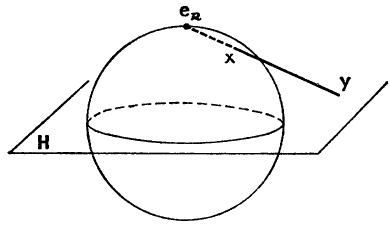
\includegraphics[keepaspectratio]{images/part001_990d2877.jpg}}\\
Figure 3.

If we denote by A the complement of \(\{e_{n}\}\) in \(S_{n-1}\) , these formulas show that we have thus defined a homeomorphism of A onto the hyperplane H. This homeomorphism is called the stereographic projection of A onto H, or (by abuse of language) the stereographic projection of \(S_{n-1}\) onto H; \(e_{n}\) is the vertex of the projection, H the hyperplane of projection. More generally, if \(H'\) is any hyperplane passing through o (a diametral hyperplane of \(B_{n}\) ) and if a is one of the points of intersection of \(S_{n-1}\) and the line orthogonal to \(H'\) passing through o, we can define in the same way the stereographic projection with vertex a onto the hyperplane of projection \(H'\) ; in any case this projection can be brought back to the preceding one by an orthogonal transformation which transforms \(H'\) into H and a into \(e_{n}\) .

PROPOSITION 4. If \(n > 1\) , the Euclidean sphere \(S_{n-1}\) is homeomorphic to the space \(\mathbf{R}^{n-1}\) made compact by adjoining a ``point at infinity'' (Chapter I, § 9, no. 8, Theorem 4).

For the stereographic projection defines a homeomorphism of the complement of a point in \(S_{n-1}\) onto a hyperplane of \(R^{n}\) , which is homeomorphic to \(R^{n-1}\) .

COROLLARY 1. The sphere \(S_{n}\) is homeomorphic to the quotient space of the ball \(B_{n}\) obtained by identifying all the points of the sphere \(S_{n-1}\) .

The ball \(B_{n}\) is a regular space (Chapter I, § 8, no. 4); hence the quotient space F of \(B_{n}\) obtained by identifying all the points of \(S_{n-1}\) is Hausdorff (Chapter I, § 8, no. 6, Proposition 15). Since \(B_{n}\) is compact, so is F, and F is therefore homeomorphic to an open ball of n dimensions made compact by adjoining a point at infinity, by Alexandroff's theorem (Chapter I, § 9, no. 8, Theorem 4). The result therefore follows from Propositions 2 and 4.

COROLLARY 2. The circle \(\mathbf{S}_1\) is homeomorphic to the torus \(\mathbf{T}\) .

In Chapter VIII, § 2, no. 1, we shall obtain this result again as a consequence of a more precise theorem.

PROPOSITION 5. If \(n > 1\) , the Euclidean sphere \(\mathbf{S}_{n-1}\) is connected and locally connected, and every point of it has an open neighbourhood homeomorphic to \(\mathbf{R}^{n-1}\) .

The complement of a point in \(S_{n-1}\) is a connected dense set, and therefore (Chapter I, § 11, no. 1, Proposition 1) \(S_{n-1}\) is connected. To see that every point has a neighbourhood homeomorphic to \(R^{n-1}\) , we have only to project stereographically from a vertex other than the given point.

From this proposition and from Proposition 3 of no. 3 it follows that \(\mathbf{R}_n^*\) , being the product of two connected spaces, is connected (Chapter I, § 11, no. 4, Proposition 8; cf.~§ 1, Exercise 10).

The intersection of \(S_{n-1}\) and a closed (resp. open) half-space determined by a diametral hyperplane of \(B_{n}\) is called a closed (resp. open) hemisphere of \(S_{n-1}\) . By stereographic projection onto the diametral hyperplane, the closed (resp. open) hemisphere which does not contain the vertex of projection is mapped onto a closed (resp. open) ball of n - 1 dimensions, to which it is therefore homeomorphic.

If n = 2, we say ``semicircle'' instead of ``hemisphere''.

\section{REAL PROJECTIVE SPACES}

In this section we shall need to invoke constantly the notions and results on quotient spaces (Chapter I, § 3), and in particular the following two properties, which for convenience we state as lemmas:

Let E be a topological space, R an equivalence relation on E, A a subset of E, \(R_{A}\) the equivalence relation induced on A by R and let f be the canonical mapping of E onto E/R. Then:

LEMMA 1. If every open (resp. closed) set in A which is saturated with respect to \(R_{A}\) is the trace on A of an open (resp. closed) set in E which is saturated with respect to R, then the quotient space \(A/R_{A}\) is homeomorphic to the subspace \(f(A)\) of E/R. This is so in particular if A is open or closed in E and saturated with respect to R.

This follows from Proposition 10 of Chapter I, § 3, no. 6.

LEMMA 2. If there is a continuous mapping \(g\) of \(\mathbf{E}\) onto \(\mathbf{A}\) such that, for all \(x \in \mathbf{E}\) , \(g(x)\) belongs to the equivalence class of \(x\) , then the quotient space \(\mathrm{A} / \mathrm{R}_{\mathbf{A}}\) is homeomorphic to \(\mathbf{E} / \mathbf{R}\) .

This is Corollary 2 of Proposition 10 of Chapter I, § 3, no. 6.

\subsection{TOPOLOGY OF REAL PROJECTIVE SPACES}

We recall the following definitions from algebra: given a division ring or a field \(\mathbf{K}\) , the set of lines passing through \(o\) (i.e.~vector subspaces of dimension 1) in the left vector space \(\mathbf{K}_s^{n+1}\) over \(\mathbf{K}\) is called left projective space of \(n\) dimensions over \(\mathbf{K}\) , and is denoted by \(\mathbf{P}_n(\mathbf{K})\) .

If we make correspond to every line passing through o in \(K_{s}^{n+1}\) the same line with the origin omitted, we have a bijection of \(\mathbf{P}_{n}(\mathbf{K})\) onto the quotient of \(K_{n+1}^{*}\) (the complement of \(\{o\}\) in \(K_{s}^{n+1}\) ) by the following equivalence relation \(\Delta_{n}(\mathbf{K})\) between vectors x and y of \(K_{n+1}^{*}\) : ``there exists \(t \in K\) such that \(t \neq o\) and y = tx''. In what follows we shall identify \(P_{n}(\mathbf{K})\) with this quotient set. In the theory of projective spaces, we take the interval \([o, n]\) of N as index set for the coordinates of a point of \(K_{n+1}^{*}\) . The coordinates \(x_{i}\) ( \(o \leqslant i \leqslant n\) ) of any one of the points of \(K_{n+1}^{*}\) whose canonical image is \(x \in P_{n}(\mathbf{K})\) constitute what is called a system of homogeneous coordinates of the point x.

For each integer \(p\) such that \(-1 \leqslant p \leqslant n\) , the canonical image in \(\mathbf{P}_n(\mathbf{K})\) of a vector subspace of \(p + 1\) dimensions (without the origin) of \(\mathrm{K}_s^{n+1}\) is called a projective linear variety of \(p\) dimensions. A system of \(p\) points of \(\mathbf{P}_n(\mathbf{K})\) is said to be free if it consists of the canonical images of \(p\) points of \(\mathrm{K}_{n+1}^*\) which form a free system in the vector space \(\mathrm{K}_s^{n+1}\) . The projective linear variety of \(\mathbf{P}_n(\mathbf{K})\) generated by a free system of \(p + 1\) points (i.e.~the smallest projective linear variety which contains these \(p + 1\) points) has dimension \(p\) .

When K is the field R, the corresponding projective spaces can be topologized, and it is these we shall study.

DEFINITION 1. The projective space \(\mathbf{P}_n(\mathbf{R})\) endowed with the quotient topology of the topology of \(\mathbf{R}_{n+1}^*\) by the equivalence relation \(\Delta_n(\mathbf{R})\) is called real projective space of \(n\) dimensions.

The projective space \(\mathbf{P}_{1}(\mathbf{R})\) is called the real projective line, and \(\mathbf{P}_{2}(\mathbf{R})\) is called the real projective plane.

Whenever there is no risk of confusion, we shall write \(P_{n}\) and \(\Delta_{n}\) instead of \(\mathbf{P}_{n}(\mathbf{R})\) and \(\Delta_{n}(\mathbf{R})\) .

PROPOSITION 1. The projective space \(P_{n}\) is Hausdorff.

We start by showing that the relation \(\Delta_{n}\) is open (Chapter I, § 5, no. 2). Let A be an open set in \(\mathbf{R}_{n+1}^{*}\) ; to saturate A with respect to \(\Delta_{n}\) we have to take the union of the sets \(t\mathbf{A}\) homothetic to A, as \(t\) runs through the set of real numbers \(\neq 0\) ; since each of these sets is open, so is their union.

By Proposition 8 of Chapter I, § 8, no. 3, the proposition will be proved if we show that the subset M of \(\mathbf{R}_{n+1}^{*}\times\mathbf{R}_{n+1}^{*}\) defined by the relation \(\Delta_{n}\) is closed. Let then \((x,y)\) be a point of \(\mathbf{R}_{n+1}^{*}\times\mathbf{R}_{n+1}^{*}\) lying in the closure of M. If \(x=(x_{i})\) , there is an index \(i\) such that \(x_{i}\neq0\) ; hence there is a neighbourhood V of \((x,y)\) such that for every point \((x^{\prime},y^{\prime})\in\mathbf{M}\cap\mathbf{V}\) the \(i\) th coordinate \(x_{i}^{\prime}\) of \(x^{\prime}\) is not o. As \((x^{\prime},y^{\prime})\) tends to \((x,y)\) while remaining in M, \(y_{i}^{\prime}x_{i}^{\prime-1}\) tends to \(t=y_{i}x_{i}^{-1}\) ; since \(y^{\prime}=(y_{i}^{\prime}x_{i}^{\prime-1})x^{\prime}\) , we see by passing to the limit that \(y=tx\) , which shows that \((x,y)\in\mathbf{M}\) .

PROPOSITION 2. The projective space \(\mathbf{P}_{n}\) is compact and connected, and is homeomorphic to the quotient of the sphere \(\mathbf{S}_{n}\) by the equivalence relation induced on the sphere by \(\Delta_{n}\) .

Let \(\Delta_n'\) be the equivalence relation induced on \(\mathbf{S}_n\) by \(\Delta_n\) (the equivalence classes of \(\Delta_n'\) are pairs of diametrically opposite points of \(\mathbf{S}_n\) ). The mapping \(x \to x/||x||\) of \(\mathbf{R}_{n+1}^*\) onto \(\mathbf{S}_n\) is continuous, hence (Lemma 2) \(\mathbf{P}_n\) is homeomorphic to \(\mathbf{S}_n/\Delta_n'\) . Since \(\mathbf{S}_n\) is compact and connected, every Hausdorff quotient space of \(\mathbf{S}_n\) is also compact and connected (Chapter I, § 9, no. 4, Theorem 2, Corollary 1; § 11, no. 3, Proposition 7).

PROPOSITION 3. If \(n \geqslant 0\) , the projective space \(\mathbf{P}_n\) is homeomorphic to the quotient space of the ball \(\mathbf{B}_n\) obtained by identifying each point of \(\mathbf{S}_{n-1}\) with its diametrically opposite point.

Let H be the closed hemisphere of \(S_{n}\) defined by \(x_{0} \leqslant 0\) . \(P_{n}\) , which is homeomorphic to the quotient space of \(S_{n}\) by the relation \(\Delta_{n}^{\prime}\) , is also homeomorphic to the quotient of the subset H of \(S_{n}\) by the relation \(\Delta_{n}^{\prime\prime}\) induced on H by \(\Delta_{n}^{\prime}\) . For every equivalence class of \(\Delta_{n}^{\prime}\) meets H in at least one point, and therefore (Lemma 1) it is enough to verify that if we saturate with respect to \(\Delta_{n}^{\prime}\) an open subset U of H which is saturated with respect to \(\Delta_{n}^{\prime\prime}\) , we get an open subset V of \(S_{n}\) . Now if \(a = (a_{i}) \in U\) and if \(a_{0} < 0\) , there is a neighbourhood W of a in \(S_{n}\) contained in U, and the union of W and \(-W\) is a neighbourhood of a saturated with respect to \(\Delta_{n}^{\prime}\) and contained in V. If on the other hand \(a_{0} = 0\) , we have \(- a \in U\) , and there exists r \textgreater{} o such that the set of points \(x \in H\) which satisfy one or the other of the relations \(||x-a||<r, ||x+a||<r\) is contained in U; the set of points \(x\in S_{n}\) which satisfy one or the other of these relations is the neighbourhood of a which is saturated with respect to \(\Delta_{n}^{\prime}\) and is contained in V.

Observe that the quotient space \(H/\Delta_{n}^{\prime\prime}\) is obtained by identifying, in H, each point of the intersection \(S_{n-1}\) of H and the hyperplane \(x_{0}=0\) with its opposite point. To complete the proof it suffices to remark that the stereographic projection with vertex \(e_{0}\) (§ 2, no. 4) is a homeomorphism of H onto \(B_{n}\) which leaves invariant the points of \(S_{n-1}\) .

\subsection{PROJECTIVE LINEAR VARIETIES}

Every injective linear mapping \(f\) of \(\mathbf{R}^{n+1}\) into \(\mathbf{R}^{m+1}\) ( \(m \geqslant n\) ) defines, by restriction to \(\mathbf{R}_{n+1}^*\) and then by passage to the quotient with respect to the relations \(\Delta_n\) and \(\Delta_m\) (Set Theory, R, § 5, no 8), an injective mapping \(g\) of \(\mathbf{P}_n\) into \(\mathbf{P}_m\) , called a projective linear mapping. If \(\varphi\) (resp. \(\psi\) ) is the canonical mapping of \(\mathbf{R}_{n+1}^*\) onto \(\mathbf{P}_n\) (resp. \(\mathbf{R}_{m+1}^*\) onto \(\mathbf{P}_m\) ), we have \(g \circ \varphi = \psi \circ f\) , which shows that \(g\) is continuous on \(\mathbf{P}_n\) (Chapter I, § 3, no. 4, Corollary to Proposition 6). In particular, every projective linear transformation of \(\mathbf{P}_n\) (i.e.~projective linear mapping of \(\mathbf{P}_n\) onto itself) is a homeomorphism of \(\mathbf{P}_n\) onto itself.

We recall also that, if V and \(V'\) are two projective linear varieties of p dimensions in \(P_{n}\) , there exists a projective linear transformation of \(P_{n}\) which transforms V into \(V'\) . In particular, if \(p \geqslant 0\) , there exists a projective linear transformation which transforms V into a coordinate projective linear variety, that is to say the canonical image of a coordinate variety \(W'\) of \(p + 1\) dimensions (without the point o) of \(R^{n+1}\) . If we identify \(W'\) with \(R_{p+1}^{*}\) , the relation induced by \(\Delta_{n}\) on \(W'\) is precisely \(\Delta_{p}\) ; since \(W'\) is closed and saturated with respect to \(\Delta_{n}\) , Lemma 1 shows that \(V'\) is homeomorphic to \(P_{p}\) and is closed in \(P_{n}\) ; moreover, if p \textless{} n, its complement is dense in \(P_{n}\) (§ 1, no. 4, Corollary to Proposition 3). Hence:

PROPOSITION 4. Every projective linear variety of p dimensions in a projective space \(P_{n}\) is closed in \(P_{n}\) and homeomorphic to \(P_{p}\) ; if p \textless{} n its complement is dense in \(P_{n}\) .

This result is the origin of the names projective line and projective plane given to projective linear varieties of one and two dimensions in a projective space over an arbitrary division ring. We recall also that the projective linear varieties of n - 1 dimensions in \(P_{n}\) are called projective hyperplanes; every projective hyperplane is identical with the set of points whose homogeneous coordinates satisfy a relation of the form \(\sum_{i=0}^{n}a_{i}x_{i}=0\) , where the \(a_{i}\) are not all zero (the ``equation'' of the hyperplane).

\pandocbounded{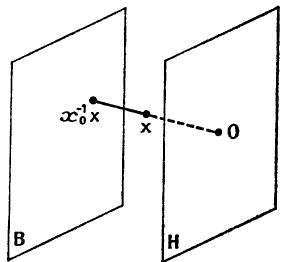
\includegraphics[keepaspectratio]{images/part001_d597a17f.jpg}}\\
Figure 4.

PROPOSITION 5. In a projective space \(\mathbf{P}_n\) ( \(n \geqslant 0\) ), the complement of a projective hyperplane H is homeomorphic to \(\mathbf{R}^n\) .

By making a projective linear transformation we may assume that H is the hyperplane whose equation is \(x_{0}=0\) . The set A of points \(\boldsymbol{x}=(x_{i})\) of \(R_{n+1}^{*}\) such that \(x_{0}\neq0\) is open and saturated with respect to \(\Delta_{n}\) ; its canonical image C in \(P_{n}\) , which is the complement of H in \(P_{n}\) , is therefore homeomorphic to the quotient of A by the equivalence relation \(\Theta\) induced on A by \(\Delta_{n}\) (Lemma 1). Let B be the hyperplane whose equation is \(x_{0}=1\) in \(R^{n+1}\) . To each point \(x\in A\) let correspond the point \(x_{0}^{-1}x\) where the line through o and x cuts B (Fig. 4); in this way we define a continuous mapping g of A onto B such that \(g(x)\) is the only point of B congruent to x modulo \(\Theta\) . It follows that B is homeomorphic to A/ \(\Theta\) (Lemma 2), hence to C; since B is homeomorphic to \(R^{n}\) , the proof is complete.

COROLLARY. Every point of \(P_{n}\) has an open neighbourhood homeomorphic to \(R^{n}\) . It follows in particular that the real projective spaces are locally connected (this follows also from Chapter I, § 11, no. 6, Proposition 12).

\subsection{EMBEDDING REAL NUMBER SPACE IN PROJECTIVE SPACE}

Proposition 5 of no. 2 shows that if we are given a projective hyperplane H in \(P_{n}\) ( \(n \geqslant 0\) ), there is a homeomorphism of \(R^{n}\) onto the complement \(\complement H\) of this hyperplane. Once H has been chosen it is often convenient to identify \(R^{n}\) and \(\complement H\) by means of the homeomorphism defined in Proposition 5; the projective hyperplane H is then said to be ``at infinity'', and so are its points and subsets. Usually one takes H to be the ``coordinate'' hyperplane whose equation is \(x_{0}=0\) , and then the point \(z=(z_{i})\) of \(R^{n}\) is identified with the point of \(P_{n}\) whose homogeneous coordinates are \(1, z_{1}, z_{2}, \ldots, z_{n}\) .

Once this identification has been made, the closure in \(P_{n}\) of any affine linear variety V of p dimensions in \(R^{n}\) is a projective linear variety of p dimensions, not contained in the hyperplane at infinity, and identical with the projective linear variety generated by V. Conversely, every projective linear variety P of p dimensions which is not contained in the hyperplane at infinity has as its trace on \(R^{n}\) an affine linear variety of p dimensions, whose closure in \(P_{n}\) is P.

In the particular case \(n = 1\) , the hyperplane at infinity is a point; since \(\mathbf{P}_1\) is compact, it follows from Alexandroff's theorem (Chapter I, §9, no. 8, Theorem 4) that \(\mathbf{P}_1\) is homeomorphic to the space \(\tilde{\mathbf{R}}\) obtained by compactifying the locally compact space \(\mathbf{R}\) by the adjunction of a point (the ``point at infinity''). By Proposition 4 of §2, no. 4, we see also that the real projective line \(\mathbf{P}_1(\mathbf{R})\) is homeomorphic to the circle \(\mathbf{S}_1\) and to the torus \(\mathbf{T}\) .

On the other hand, if \(n > 1\) , \(\mathbf{P}_n(\mathbf{R})\) is not homeomorphic to \(\mathbf{S}_n\) , as we shall see later (cf.~Exercise 4).

The ``point at infinity'' of the space \(\tilde{R}\) is denoted by \(\infty\) , with no sign attached. It is important not to confuse \(\tilde{R}\) with the extended real line \(\overline{R}\) defined in Chapter IV, § 4, which has two ``points at infinity''; indeed \(\tilde{R}\) is homeomorphic to the quotient space of \(\overline{R}\) obtained by identifying the two points \(+\infty\) and \(-\infty\) .

\subsection{APPLICATION TO THE EXTENSION OF REAL-VALUED FUNCTIONS}

Since \(\mathbf{R}\) can be considered as a subset of \(\tilde{\mathbf{R}}\) , every mapping of a set \(\mathbf{E}\) into \(\mathbf{R}\) (i.e.~every real-valued function on \(\mathbf{E}\) ) can be considered as a mapping of \(\mathbf{E}\) into \(\tilde{\mathbf{R}}\) ; in particular, if \(\mathbf{E}\) is a subset of a topological space \(\mathbf{F}\) and \(f\) is a mapping of \(\mathbf{E}\) into \(\mathbf{R}\) , it may happen that at some points of the closure \(\overline{\mathbf{E}}\) of \(\mathbf{E}\) , \(f(x)\) tends to the limit \(\infty\) as \(x\) tends to one of these points while remaining in \(\mathbf{E}\) ; we may then extend the function \(f\) by continuity by assigning it the value \(\infty\) at these points (Chapter I, § 8, no. 5, Theorem 1).

Consider in particular the case where E is a subset of \(R^{n}\) , the space \(R^{n}\) itself being considered as embedded in projective space \(P_{n}\) ; if we suppose that the hyperplane at infinity is \(x_{0}=0\) , a real-valued function f defined on E may be identified with the mapping

\[
(x _ {0}, x _ {1}, x _ {2}, \ldots , x _ {n}) \rightarrow f \left(\frac {x _ {1}}{x _ {0}}, \frac {x _ {2}}{x _ {0}}, \ldots , \frac {x _ {n}}{x _ {0}}\right)
\]

of E into \(\tilde{R}\) ; from what has been said in the previous paragraph it may be possible to extend this function, not only to some points of \(R^{n}\) in the closure of E, but also to some of the ``points at infinity'' of \(P_{n}\) in the closure of E.

Let us show that we obtain in this way, for example, the extension by continuity to the whole of \(\tilde{\mathbf{R}}\) of a rational function of a real variable, already defined in algebra. Let us identify \(\tilde{\mathbf{R}}\) and \(\mathbf{P}_1\) , every real number \(x \in \mathbb{R}\) being identified with the point whose homogeneous coordinates are (1, x), and the point \(\infty\) with the point whose homogeneous coordinates are (0,1). Let \(u(x)/v(x)\) be a rational function, \(u\) and \(v\) being two coprime polynomials of degrees \(m\) and \(n\) respectively; if we suppose for example that \(m \leqslant n\) , and if we put \(u_1(x,y) = x^n u(y/x)\) , \(v_1(x,y) = x^n v(y/x)\) , the rational function \(u/v\) may be considered as the restriction, to the set of real numbers \(x\) such that \(v(x) \neq 0\) , of the mapping \((x,y) \to (v_1(x,y), u_1(x,y))\) . In other words, we extend \(u/v\) by continuity, by giving it the value \(\infty\) at those points \(x \in \mathbb{R}\) where \(v(x) = 0\) , and by giving it at the point \(\infty\) the value \(0\) if \(m < n\) , the value \(\infty\) if \(m > n\) , and the value of the ratio of the leading coefficients if \(m = n\) .

In particular, the function \(1 / x\) can be extended to the point \(o\) by taking the value \(\infty\) there, to \(\infty\) by taking the value \(o\) there; this extended function is evidently a homeomorphism of \(\tilde{\mathbf{R}}\) onto itself. The same is true of the homographic function \((ax + b) / (cx + d)\) when \(ad - bc \neq o\) .

Likewise, if \(n\) is an integer \(> 0\) , the function \(x^n\) extends to the point \(\infty\) by taking the value \(\infty\) there.

On the other hand, it is in general impossible to extend by continuity a rational function of two real variables either to the space \(\mathbf{P}_1 \times \mathbf{P}_1\) or to the space \(\mathbf{P}_2\) (cf.~Exercise 5).

\subsection{SPACES OF PROJECTIVE LINEAR VARIETIES}

Given a division ring K, the set \(\mathbf{P}_{n,p}(\mathbf{K})\) of projective linear varieties of \(p \geqslant 0\) dimensions of the left projective space \(\mathbf{P}_{n}(\mathbf{K})\) is clearly in one-to-one correspondence with the set of vector subspaces of \(p + 1\) dimensions of the left vector space \(K_{s}^{n+1}\) . Let \(L_{n+1, p+1}(\mathbf{K})\) denote the set of free systems \((x_{k})_{1 \leqslant k \leqslant p+1}\) of \(p + 1\) vectors of \(K_{s}^{n+1}\) ; then the set \(\mathbf{P}_{n,p}(\mathbf{K})\)

is again in one-to-one correspondence with the quotient of \(\mathbf{L}_{n+1,p+1}(\mathbf{K})\) by the equivalence relation \(\Delta_{n,p}(\mathbf{K})\) : `` \((\mathbf{x}^{k})\) and \((\mathbf{y}^{k})\) generate the same vector subspace of \(p+1\) dimensions of \(K_{s}^{n+1}\) ''. In what follows we shall identify \(\mathbf{P}_{n,p}(\mathbf{K})\) with this quotient set. On the other hand, if to each free system \((\mathbf{x}_{k})\) of \(p+1\) vectors of \(K_{s}^{n+1}\) we make correspond the matrix X of \(p+1\) rows and \(n+1\) columns for which \(x_{k}\) is the kth row ( \(1\leqslant k\leqslant p+1\) ), we have a one-to-one correspondence between \(L_{n+1,p+1}(\mathbf{K})\) and the set of all matrices of \(p+1\) rows and \(n+1\) columns which are of rank \(p+1\) ; we shall identify \(L_{n+1,p+1}(\mathbf{K})\) with this set of matrices, and the relation \(\Delta_{n,p}(\mathbf{K})\) between two matrices X, Y is then the following: `` there exists a non-singular square matrix T of order \(p+1\) such that Y = T.X''.

In what follows we shall take K to be the field R, and we shall omit the letter K in the notation above. We can define a topology on \(P_{n,p}\) by a process which generalizes the definition of the topology of real projective spaces. Namely, \(L_{n+1, p+1}\) is contained in the space \(M_{p+1, n+1}\) of all matrices of \(p + 1\) rows and \(n + 1\) columns with real elements; we endow \(L_{n+1, p+1}\) with the topology induced by the topology of this matrix space (§ 1, no. 6).

DEFINITION 2. The space \(\mathbf{P}_{n,p}\) which is the quotient of the topological space \(\mathbf{L}_{n+1,p+1}\) by the equivalence relation \(\Delta_{n,p}\) is called the space of projective linear varieties of \(p\geqslant0\) dimensions in real projective space \(\mathbf{P}_{n}\) .

We shall use the following notation: given a matrix X of \(p + 1\) rows and \(n + 1\) columns, and any strictly increasing sequence

\[
\sigma = (i _ {1}, \dots , i _ {p + 1})
\]

of \(p + 1\) indices belonging to the interval \([0, n]\) of \(\mathbf{N}\) , we denote by \(X_{\sigma}\) the square submatrix of \(X\) formed by the columns whose indices are \(i_1, i_2, \ldots, i_{p+1}\) . We denote by \(\mathbf{A}_{\sigma}\) the subset of \(\mathbf{L}_{n+1, p+1}\) consisting of these matrices \(X\) such that \(X_{\sigma}\) is non-singular. By Proposition 6 of § 1, no. 6, \(\mathbf{A}_{\sigma}\) is a dense open set in \(\mathbf{M}_{p+1, n+1}\) , and the function \(X \to X_{\sigma}^{-1}\) is continuous on \(\mathbf{A}_{\sigma}\) .

A geometrical interpretation of the set \(A_{\sigma}\) is as follows: let \(E_{\sigma}\) be the vector subspace of \(R^{n+1}\) generated by the vectors \(e_{i}\) of the canonical basis such that \(i \in \sigma\) , and let \(E_{\sigma}'\) be the complementary subspace generated by the \(e_{i}\) such that \(i \notin \sigma\) ; then to say that a matrix x belongs to \(A_{\sigma}\) means that the projections on \(E_{\sigma}\) of its \(p + 1\) rows of \(x_{k}\) form a free system, or again that the vector subspace generated by the \(x_{k}\) is a complement of \(E_{\sigma}'\) (or that its intersection with \(E_{\sigma}'\) consists only of o).

PROPOSITION 6. The space \(\mathbf{P}_{n,p}\) is Hausdorff.

We show first that the relation \(\Delta_{n,p}\) is open. If U is an open set in \(L_{n+1,p+1}\) , to saturate U with respect to \(\Delta_{n,p}\) we have to take the union of the images of U under the mapping \(X \to T \cdot X\) , where T runs through the set of non-singular square matrices of order \(p + 1\) ; since each of these mappings is bicontinuous, all these images are open sets and therefore so is their union.

By Proposition 8 of Chapter I, § 8, no. 3, the proof will be complete if we show that the subset N of \(L_{n+1,p+1} \times L_{n+1,p+1}\) , defined by \(\Delta_{n,p}\) , is closed. Let \((X,\mathcal{Y})\) be a point of the product space which lies in the closure of N, and let \(\sigma\) be a sequence of indices such that \(X_{\sigma}\) is non-singular: since \(A_{\sigma}\) is open, there is a neighbourhood V of \((X,\mathcal{Y})\) such that, for each pair \((X',\mathcal{Y}') \in \mathrm{N} \cap \mathrm{V}\) , the matrix \(X'_{\sigma}\) is non-singular; as \((X',\mathcal{Y}')\) tends to \((X,\mathcal{Y})\) while remaining in N, the matrix \(Y'_{\sigma}X_{\sigma}^{\prime -1}\) therefore tends to \(T = Y_{\sigma}X_{\sigma}^{-1}\) ; since we have \(Y' = (Y'_{\sigma}X_{\sigma}^{\prime -1})X'\) , we see by passing to the limit that Y = T.X, and the proof is complete.

PROPOSITION 7. The space \(\mathbf{P}_{n,p}\) is compact.

It is enough to show that there is a compact subspace of \(L_{n+1, p+1}\) which meets every equivalence class mod \(\Delta_{n,p}\) in at least one point; for \(P_{n,p}\) is then the image of this subspace under the canonical mapping of \(L_{n+1, p+1}\) onto \(P_{n,p}\) , and is therefore compact (Chapter I, § 9, no. 4, Theorem 2).

Let \(\mathbf{V}_{n+1, p+1}\) be the subspace of \(\mathbf{L}_{n+1, p+1}\) whose elements are the systems \((\boldsymbol{x}_k)\) of \(p + 1\) vectors forming an orthonormal Euclidean basis of the vector subspace they generate that is to say such that \((x_h | x_k) = 0\) whenever \(h \neq k\) , \((x_h | x_h) = 1\) for \(1 \leqslant h \leqslant p + 1\) . Every vector subspace of \(p + 1\) dimensions of \(\mathbf{R}^{n+1}\) has such a basis and therefore every class mod. \(\Delta_{n,p}\) meets \(\mathbf{V}_{n+1, p+1}\) . On the other hand, the matrices \(X = (x_{ij})\) of \(\mathbf{V}_{n+1, p+1}\) are defined by the relations

\[
\sum_ {j = 0} ^ {n} x _ {i j} ^ {2} = 1 (1 \leqslant i \leqslant p + 1),
\]

\[
\sum_ {j = 0} ^ {n} x _ {i j} x _ {k j} = 0 \quad (i \neq k);
\]

therefore they form a closed set in \(M_{p+1, n+1}\) ; and since these relations imply that \(|x_{ij}| \leqslant 1\) for each pair of indices \((i, j)\) , this set is bounded and hence compact.

PROPOSITION 8. \(\mathbf{P}_{n,p}\) is connected and locally connected, and every point has an open neighbourhood homeomorphic to \(\mathbf{R}^{(p+1)(n-p)}\) .

For every (strictly increasing) sequence of indices \(\sigma\) , the set \(\mathbf{A}_{\sigma}\) is open in \(\mathbf{L}_{n+1, p+1}\) and saturated with respect to \(\Delta_{n,p}\) ; its canonical image

\(C_{\sigma}\) in \(P_{n,p}\) is therefore an open set homeomorphic to the quotient of \(A_{\sigma}\) by the equivalence relation \(\Theta_{\sigma}\) induced on \(A_{\sigma}\) by \(\Delta_{n,p}\) (Lemma 1).

Let \(\mathbf{B}_{\sigma}\) be the subset of \(\mathbf{A}_{\sigma}\) consisting of matrices \(X\) such that \(X_{\sigma}\) is the unit matrix of order \(p + 1\) ; the elements of \(X\) other than those of \(X_{\sigma}\) are then arbitrary, and therefore \(\mathbf{B}_{\sigma}\) is homeomorphic to the space \(\mathbf{R}^{(p + 1)(n - p)}\) . To each matrix \(X \in \mathbf{A}_{\sigma}\) let us make correspond the matrix \(\Upsilon = X_{\sigma}^{-1}X\) , which belongs to \(\mathbf{B}_{\sigma}\) ; then we have defined a continuous mapping \(g\) of \(\mathbf{A}_{\sigma}\) onto \(\mathbf{B}_{\sigma}\) , such that \(g(X)\) is the only matrix of \(\mathbf{B}_{\sigma}\) congruent to \(X\) mod \(\Theta_{\sigma}\) . It follows that \(\mathbf{B}_{\sigma}\) is homeomorphic to \(\mathbf{A}_{\sigma}/\Theta_{\sigma}\) (Lemma 2), hence to \(\mathbf{C}_{\sigma}\) .

The set \(C_{\sigma}\) is therefore connected. Since \(A_{\sigma}\) is dense in \(L_{n+1, p+1}\) , \(C_{\sigma}\) is dense in \(P_{n, p}\) and therefore \(P_{n, p}\) is also connected (Chapter I, § 11, no. 1, Proposition 1). On the other hand, every point of \(P_{n, p}\) belongs to \(C_{\sigma}\) for at least one sequence of indices \(\sigma\) , and therefore has an open neighbourhood homeomorphic to \(\mathbf{R}^{(p+1)(n-p)}\) .

The matrix \(Y=g(X)\) can be interpreted as follows: let us suppose for the sake of simplicity that the sequence \(\sigma\) consists of the \(p+1\) indices n-p, \(n-p+1\) , \(\ldots\) , n, and let \(a_{ij}\) ( \(1\leqslant i\leqslant p+1\) , \(o\leqslant j\leqslant n-p-1\) ) denote the elements of the first n-p columns of y; then the vector subspace of \(R^{n+1}\) generated by the rows of x is that defined by the equations

\[
x _ {j} = \sum_ {i = 1} ^ {p + 1} a _ {i j} x _ {n - p + i - 1} \quad (0 \leqslant j \leqslant n - p - 1).
\]

\subsection{GRASSMANNIANS}

If K is a field and X is any matrix of \(\mathrm{L}_{n+1,p+1}(\mathrm{K})\) , let \(c_{\sigma}(X)\) denote the determinant of \(X_{\sigma}\) ; in this way, to each matrix X of \(\mathrm{L}_{n+1,p+1}(\mathrm{K})\) correspond

\[
h = \binom {n + 1} {p + 1}
\]

determinants, not all zero (the components of the exterior product of the \(p + 1\) rows of \(X\) ). If we make correspond to \(X\) the point of the projective space \(\mathbf{P}_{h-1}(\mathbf{K})\) whose homogeneous coordinates are the \(c_{\sigma}(X)\) , we have defined a mapping of \(\mathbf{L}_{n+1,p+1}(\mathbf{K})\) into \(\mathbf{P}_{h-1}(\mathbf{K})\) , compatible with the relation \(\Delta_{n,p}(\mathbf{K})\) ; passing to the quotient, we have therefore a mapping \(f\) of \(\mathbf{P}_{n,p}(\mathbf{K})\) into \(\mathbf{P}_{h-1}(\mathbf{K})\) . The image \(\mathbf{G}_{n,p}(\mathbf{K})\) of \(\mathbf{P}_{n,p}(\mathbf{K})\) under this mapping is called the Grassmannian of indices \(n\) , \(p\) . We recall also that the mapping \(f\) is injective, for if \(X\) is a matrix such that \(X_{\sigma}\) is non-singular, the matrix \(\Upsilon = X_{\sigma}^{-1}X\) of \(\mathbf{B}_{\sigma}\) which corresponds to the class of \(X\) mod. \(\Delta_{n,p}(\mathbf{K})\) is the matrix \((d_{ij}/c_{\sigma}(X))\) ( \(1 \leqslant i \leqslant p + 1\) , \(0 \leqslant j \leqslant n\) ), where \(d_{ij}\) denotes the determinant of the matrix obtained from \(X_{\sigma}\) by replacing the ith column of \(X_{\sigma}\) by the jth column of X {[}which implies that \(d_{ij}\) is, up to sign, equal to one of the \(c_{\tau}(X)\) {]}.

When \(\mathbf{K}\) is the field \(\mathbf{R}\) , this mapping \(f\) is evidently continuous. The inverse mapping \(g\) is also continuous; for the elements of a matrix belonging to \(\mathbf{B}_{\sigma}\) are rational functions of the homogeneous coordinates of the point of the Grassmannian to which it corresponds; since \(f(\mathbf{B}_{\sigma}) = \mathbf{B}_{\sigma}'\) is the set of points of \(\mathbf{G}_{n,p}\) whose homogeneous coordinate with index \(\sigma\) is not \(0\) , it is an open set in \(\mathbf{G}_{n,p}\) ; hence \(g\) is continuous at every point of \(\mathbf{B}_{\sigma}'\) , and since every point of \(\mathbf{G}_{n,p}\) belongs to at least one set \(\mathbf{B}_{\sigma}'\) , \(g\) is continuous at every point. Thus:

PROPOSITION 9. The Grassmannian \(\mathbf{G}_{n,p}\) is homeomorphic to the space \(\mathbf{P}_{n,p}\) .

We recall finally that the Grassmannians \(\mathbf{G}_{n,p}(\mathbf{K})\) and \(\mathbf{G}_{n,n-p-1}(\mathbf{K})\) are subsets of the same projective space \(\mathbf{P}_{h-1}(\mathbf{K})\) and can be transformed into the other by a projective linear transformation; it follows that \(G_{n,p}\) and \(G_{n,n-p-1}\) are homeomorphic.
